\documentclass[12pt,a4paper]{article}
\usepackage[utf8]{inputenc}
\usepackage[english]{babel}
\usepackage[T1]{fontenc}
\usepackage{amsmath}
\usepackage{amsfonts}
\usepackage{amssymb}
\usepackage{subcaption}
\usepackage{makeidx}
\usepackage{graphicx}
\usepackage{fourier}
\usepackage{listings}
\usepackage{color}
\usepackage{hyperref}
\usepackage[left=2cm,right=2cm,top=2cm,bottom=2cm]{geometry}
\author{Tommy Müller, Marcus Dittrich, Vincent Noculak}
\title{Holographie}


\lstset{language=C++,
	keywordstyle=\bfseries\color{blue},
	commentstyle=\itshape\color{red},
	stringstyle=\color{green},
	identifierstyle=\bfseries,
	frame=single}
\begin{document}

\maketitle
\newpage
\tableofcontents
\newpage
	
\section{Theorie}

\subsection{Einleitung}

Die Holographie ist ein von Dennis Gabor(1900-1979) entwickeltes Verfahren zur räumlichen Abbildung von Objekten. Im Gegensatz zur herkömmlichen Photographie, welche nur Informationen über die Intensität des Lichtwellenfeldes eines abgebildeten Gegenstandes aufnimmt, ermöglicht Holographie die Darstellung räumlicher Charakteristika. Dafür werden Phase und Amplitude durch Hinzunahme einer Referenzwelle gespeichert.Grundbedingung hierfür ist die Kohärenz des Lichtes um eine feste Phasenbeziehung zwischen Objekt und Referenzwelle zu erhalten. Die Phasenbeziehung ist dann aus dem entstehenden Interferenzmuster auf der Photoplatte, zwischen Objekt- und Referenzwelle, abzulesen. Das erhaltene Bild hat zunächst keine Ähnlichkeit mit dem Orginalobjekt, es muss erst wieder speziell beleuchtet werden um ein dreidimensionales Abbild des Objektes zu erhalten. Da Objekt- und Referenzwelle die gleiche Wellenlänge besitzen, dürfen die Bauteile des Versuchsaufbaus innerhalb der Belichtungsdauer nur um einen Bruchteil ihrer Wellenlänge ($\lambda/4$) bewegt werden, um das Interferenzmuster nicht zu verzerren. Da meist ein HeNe-Laser mit einer Wellenlänge von $\lambda = 632nm$ verwendet wird, reichen leichte Erschütterungen aus, um das entstehende Bild unbrauchbar zu machen. Deswegen benötigen wir ein Instrument, um unseren Aufbau auf die nötige Stabilität zu Prüfen. 

\subsection{Michelson-Interferometer}

In unserem Aufbau wir dafür ein Michelson-Interferometer benutzt. Im Allgemeinen besteht die Funktionsweise eines Interferometers darin, eine einfallende Lichtwelle in zwei Wellen zu teilen. Diese durchlaufen dann unterschiedlich lange Wegstrecken, wodurch sich eine Phasenverschiebung zwischen beiden Wellen ergibt. Werden beide Wellen wieder zusammengefügt, kommt es zur Interferenz. \begin{figure}[h]
	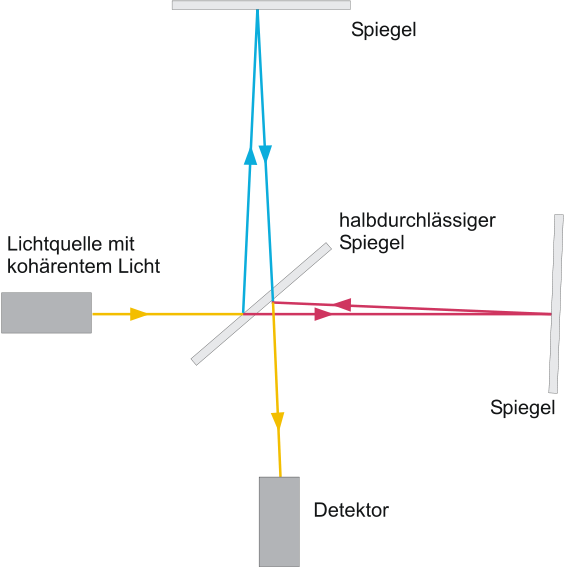
\includegraphics[scale = 0.5]{Michelson.png}
	\centering
	\caption{Schematischer Aufbau eines Michelson-Interferometers}
	\label{11}
\end{figure}Im Michelson-Interferometer wird der einfallende Strahl aus einer koherenten Lichtquelle im Zentrum des Aufbaus durch einen halb durchlässigen Spiegel geteilt. Anschließen werden die beiden Strahlen reflektiert und im Zentrum wieder zusammengefügtum auf dem Detektor zu interferieren. Ist auf dem Detektor ein Interferenzmuster zu erkennen, so ist der Weglängenunterschied den beide Wellen durchlaufen haben innerhalb der Kohärenzlänge der Strahlungsquelle. Minimale Veränderungen der Weglänge sind anhand von Änderungen des Interferenzmusters auf dem Detektor zu erkennen. Somit kann über die Beobachtung der Interferenzmuster die Stabilität des Aufbaus abgeschätzt werden. Der schematische Aufbau des Michelson-Interferometers wird in Figure $\ref{11}$ dargestellt.

\subsection{Physikalische Grundlagen}

\subsubsection{Kohärenz}

Als Kohärenz wird die Eigenschaft einer Lichtquelle bezeichnet, mit sich selber interferieren zu können. Bedingung dafür ist, das die Lichtquelle monochromatisch ist und eine feste Phasenbeziehung zwischen den einzelnen Teilwellen besteht.

\subsubsection{Interferenz und Beugung}

Als Interferenz bezeichnet man die Überlagerung zweier kohärenter Wellen. Dabei gibt es zwei Extremfälle, konstruktive und destruktive Interferenz. Bei der konstruktiven Interferenz liegen Minima und Maxima übereinander, wodurch die Amplituden addiert werden. Bei destruktiver Interferenz sind die beiden Wellen um $\pi/2$ zueinander verschoben, wodurch sich die Wellenfunktionen bei gleicher Amplitude auslöschen. Schickt man einen kohärenten Lichtstrahl durch ein optisches Gitter, dessen Gitterkonstante in etwa der Wellenlänge des einfallenden Lichts entspricht, so ergibt sich auf dem Schirm hinter dem Gitter ein Interferenzmuster. Diese Muster entstehen durch Interferenz der, am Gitter neu entstehenden Wellen, miteinander. Des Weiteren gibt es Beugung am Kristallgitter, bei dem Interferenz durch Reflexion an den regelmäßig angeordneten Kristallgittern entsteht. Dafür lässt sich die Bragg-Bedingung festhalten, welche für die Reflexionsholographie von Bedeutung sein wird:

\begin{equation}
2k \frac{\lambda}{2} = |2d sin \nu|
\label {1}
\end{equation}
	
\subsection{Varianten der Holographie}

Es gibt mehrere Möglichkeiten Holographie zu betreiben, welche sich Grundlegend durch ihren Aufbau unterscheiden. Die Zwei Ausgangsmodelle sind die Transmissions- und Reflexionsholographie, welche wir in den folgenden Absätzen näher erläutern wollen. 

\subsubsection{Transmissionsholographie}

\begin{figure}[h]
	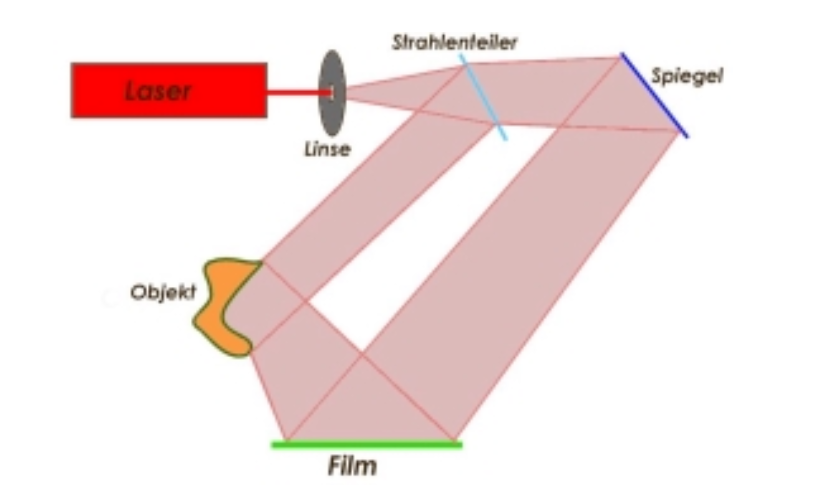
\includegraphics[scale = 0.5]{Trans.png}
	\centering
	\caption{Möglicher Aufbau zur Aufnahme eines Transmissionshologramms}
	\label{22}
\end{figure}

In Figure $\ref{22}$ wird eine Möglichkeit des schematischen Aufbaus zur Transmissionsholographie dargestellt. Eine kohärente Lichtquelle emittiert  Licht, welches in einem halb durchlässigen Spiegel geteilt wird. Der eine Strahl trifft auf das zu untersuchende Objekt, von welchem es auf die Photoplatte reflektiert wird. Der sog. Referenzstrahl wird hinter dem Strahlenteiler unverändert auf die Platte geleitet. Um den Vorgang theoretisch zu beschreiben muss man Objekt- und Referenzwelle überlagern und aus der Summe der Amplituden die Intensität bestimmen. An einem Ort (x,y) auf der Photoplatte ergibt sich für die elektrische Feldstärke:
\begin{equation}
\ E(x,y,t) = O(x,y,t) + R(x,y,t)
\label {1}
\end{equation}
geht man davon aus, das für $O(x,y,t)=O(x,y)*e^{-i\omega t}$ und $R(x,y,t)=R(x,y)*e^{-i\omega t}$ gilt, so ergibt sich für die Intensität:

\begin{equation}
\ I(x,y) = |O(x,y) + R(x,y)|^{2} = (O+R)(O+R)^{*} = RR^{*} + OO^{*} + R^{*}O + O^{*}R
\label {1}
\end{equation}
Bei $R^{*}$ und $ O^{*}$ handelt es sich um komplex konjugierte Amplituden. Während der kompletten Belichtungszeit reagiert die Photoplatte auf die einfallende Energie pro Fläche und setzt dies in eine Schwärzung der Photoplatte mit Veränderung des Brechungsindexes am Ort (x,y) um. Die Belichtung B [Energie/Fläche] ist über folgendes Integral bestimmt, wobei $t_{b}$ die Belichtungszeit ist:
\begin{equation}
\ B(x,y) = \int_{0}^{t_{b}}I(x,y) 
\label {1}
\end{equation}
Die Belichtung führt zu einer komplexen Amplitudentransmission des Negativs. Dafür lässt sich der komplexe Amplitudentransmissionsgrad $\tau$ bestimmen:
\begin{equation}
\tau = \frac{E_{a}}{E_e}  = Te^{i\psi} = |\tau|e^{i\psi}
\label {1}
\end{equation}
$E_{a}$ und $E_{e}$ sind hierbei die einfallende und die auslaufende Welle. Für den komplexen Amplitudentrainsmissionsgrad gilt als Funktion des Ortes auf der Photoplatte:
\begin{equation}
\tau = \frac{E_{a}}{E_e} = \tau(x,y) = T(x,y)e^{i\psi(x,y)} 
\label {1}
\end{equation}
Es gibt zwei gängige Arten zur Betrachtung des Problems, bei der einen nimmt man $\psi$ = const. an, dem sog. Amplitudenhologramm. Bei der anderen geht man davon aus, das T = const. und erhält das sog. Phasenhologramm. Für beide Varianten lässt sich der Verlauf von Amplitude und Phase in Abhängigkeit von der Belichtung B skizzieren, wie in Figure $\ref{33}$ $\&$ $\ref{44}$ zu sehen ist.
\begin{figure}[h]
	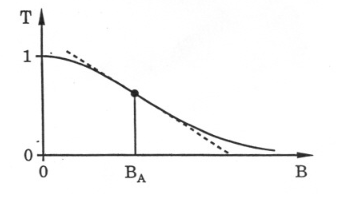
\includegraphics[scale = 0.5]{Amptrans.png}
	\centering
	\caption{Verlauf von T über B beim Amplitudenhologramm}
	\label{33}
\end{figure}
\begin{figure}[h]
	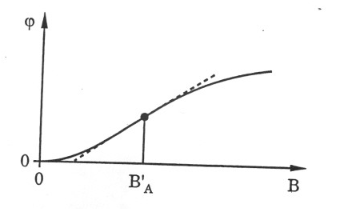
\includegraphics[scale = 0.5]{Phasentrans.png}
	\centering
	\caption{Verlauf von $\psi$ über B beim Phasenhologramm}
	\label{44}
\end{figure}

Beide Funktionen werden um einen Arbeitspunkt $B_{A}$ linear genähert. Für das Amplitudenhologramm gilt somit der Zusammenhang:

\begin{equation}
T = a- bB = a-bIt_{B}
\label {1}
\end{equation}

Für das Phasenhologramm ergibt sich für die lineare Näherung in der Umgebung des Arbeitspunktes $B_{A}$:

\begin{equation}
\psi(I) = a^{'} + b^{'}tIt_{B}
\label {1}
\end{equation}

Dies führt zu:

\begin{equation}
\tau = e^{i\psi(I)} 
\label {1}
\end{equation}

Um dafür den linearen Zusammenhang zu erhalten entwickelt man die Exponentialfunktion für $\psi(I) << \pi/2$ und bricht nach dem linearen Glied ab, so dass man folgenden Zusammenhang erhält:

\begin{equation}
\tau = e^{i\Psi(I)} = 1 + i\Psi(I)
\label {3}
\end{equation}

Sowohl beim Amplitudenhologramm, als auch bei Phasenhologramm gilt der Zusammenhang:

\begin{equation}
\tau(x,y) \propto I(x,y)
\label {2}
\end{equation}

Um die entwickelte Photoplatte auswerten zu können, wird der Laser auf die Platte gerichtet. Ein Teil des Lichts transmittiert durch die Platte entsprechend des Transmissionskoeffizienten $\tau$, welcher  Ortsgebunden proportional zur Intensität bei der Hologrammerzeugung ist, wie in Gleichung $\ref{2}$ beschrieben. Man erhält hinter der Hologrammfläche für das Amplitudenhologramm die komplexe Amplitude $E_{a}$:

\begin{equation}
E_{a}(x,y) = T(x,y)E_{e} = T(x,y)R = Ra-bt_{B}R(RR^{*} + OO^{*} + R^{*}O + O^{*}R)
\label {1}
\end{equation}

Die vier Terme der Gleichung haben der Reihe nach folgende Bedeutungen, die ersten beiden Terme sind die Nullte Ordnung der Referenzwelle, jeweils mit einem konstanten Faktor multipliziert. Der dritte Term ist das virtuelle Bild, welches sowohl Objektamplitude als auch Objektphase enthält, während der vierte Term das konjugierte Bild des Objektes, welcher auch als pseudoskopisch betitelt wird. Um ein möglichst gutes Bild zu erhalten, versucht man die drei Störterme, also alle bis auf das virtuelle Bild, zu minimieren. Die Rekonstruktion des Bildes mithilfe eines Phasenhologramms ist analog dazu mit dem Transmissionskoeffizienten aus Gleichung $\ref{3}$. Im Vergleich zwischen Phasen- und Amplitudenhologramm liefert das Phasenhologramm das hellere Bild, dafür hat es allerdings mehr Störeffekte. 

\subsubsection{Reflexionsholographie}

Im Gegensatz nur Transmissionsholographie treffen bei der Reflexionsholographie Objekt- und Referenzwelle von unterschiedlichen Seiten auf die Photoplatte. Des Weiteren ist diese anders beschaffen, sie besteht aus einer Gelatineschicht, welche wesentlich dicker ist, als die bei der Transmissionsholographie benutzte Photoplatte. Dadurch werden Interferenzbilder in verschiedenen Ebenen aufgenommen. Daher spricht man im Falle der Reflexionsholographie auch von Volumenhologrammen, während man Transmissionshologramme auch als Flächenhologramme bezeichnet. In Figure $\ref{55}$ wird eine Möglichkeit des schematischen Aufbaus zur Reflexionsholographie dargestellt. 
\begin{figure}[h]
	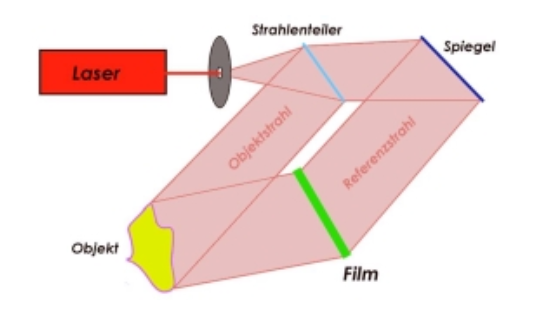
\includegraphics[scale = 0.5]{Refl.png}
	\centering
	\caption{Möglicher Aufbau zur Aufnahme eines Reflexionshologramms}
	\label{55}
\end{figure}
Dabei bilden Objekt- und Referenzstrahl innerhalb des Photomaterials stehende Wellen aus, wodurch in mehreren Ebenen ein Interferenzmuster erzeugt wird, was in Figure $\ref{66}$ schematisch dargestellt ist. Die Skizze veranschaulicht außerdem das entstehen mehrerer Netzebenen innerhalb des Photomaterials. 

\begin{figure}[h]
	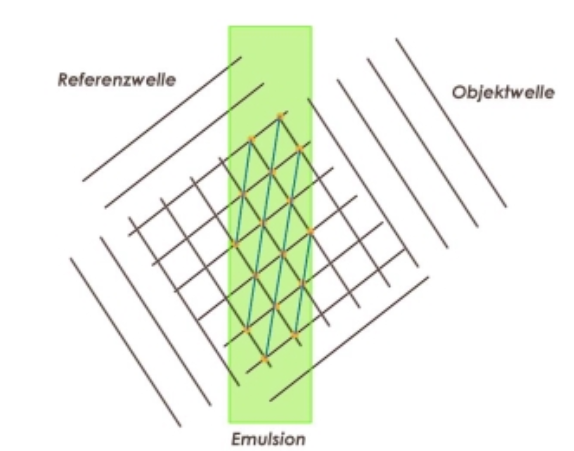
\includegraphics[scale = 0.5]{refsteh.png}
	\centering
	\caption{Entwicklung der Netzebenen innerhalb des Photomaterials}
	\label{66}
\end{figure}

Die verschiedenen Ebenen entsprechen dabei Reflexionsgittern. Der Abstand der Netzebenen zueinander wird durch die Wellenlänge $\lambda$ und Winkel des einfallenden Lichts $\nu$ bestimmt. Es gilt folgender Zusammenhang:

\begin{equation}
d = \frac{1}{2} \frac{\lambda}{|sin \nu|}
\label {1}
\end{equation}

Um das Hologramm darstellen zu können wird die Reflexion des Referenzstrahl durch das Photomaterial geschickt. Der einfallende Lichtstrahl wird an den Netzebenen nach der Bragg-Bedingung reflektiert. Wird der Einstrahlungswinkel $\nu$ variiert ist die Bedingung nicht mehr erfüllt und das Objekt kann nicht wiedergegeben werden. Die Bragg-Bedingung ermöglicht es die Rekonstruktion auch mit "weißem" Licht durchzuführen, da bestimmte Teilwellen die Bedingungen erfüllen. Dabei erhält man Licht verschiedener Wellenlängen, was zu unterschiedlichen Farbgebungen führt. 

\subsubsection{Andere Verfahren}

Reflexions- und Transmissionholograhpie sind die Grundlagen aller holographischen Verfahren. Allerdings gibt es noch einige, welche auf den Grundlagen der zuvor genannten Verfahren beruhen, sich allerdings im Versuchsaufbau unterscheiden. Eines davon ist das Denisjuk-Hologramm, benannt nach dem sowjetischen Physiker Juri Nikolajewitsch Denisjuk. Dabei handelt es sich um eine Vereinfachung der Reflexionsholographie. Hierbei wird der Laserstrahl nicht geteilt. Der Strahl wird durch eine Linse aufgeweitet und durchleuchtet als Referenzstrahl das Photomaterial. Das zu untersuchende Objekt befindet sich hinter der Photofläche und reflektiert Licht als Objektstrahl auf die Rückseite des Photomaterials. Dadurch entsteht wieder Interferenz nach dem Verfahren der Reflexionsholographie. Der schematische Aufbau lässt sich in Figure $\ref{77}$ nachvollziehen. Weitere Verfahren sind Sichtlinienholographie, Auflichtholographie, Durchlichtholographie, Weißlichtholographie,  Regenbogenholographie, die holographische Kinematographie und die digitale Holographie. 

\begin{figure}[h]
	\includegraphics[scale = 0.5]{denis.png}
	\centering
	\caption{Stabilitätsdiagramm einer Paulfalle}
	\label{77}
\end{figure}

\section{Durchführung}


\subsection{Erstellung der Hologramme}

Als erstes haben wir den Aufbau zum Erstellen der Hologramme verwendet. Das zu holografierende Objekt wurde auf einem, um 30° gekippten, Sockel in den Strahlengang gestellt. Unsere Objekte waren eine Schachfigur, Monopoly Hotel, Origami Figur und ein Happyhippo R2D2. Vor dem Sockel befand sich die Scheibe, die als Halterung für den holografischen Film diente. 
Der Laserstrahl ging zunächst durch die Scheibe und wurde dann vom Objekt gestreut. Die Objekte müssen sich für die Aufnahme möglichst nah am Film befinden, damit erstens sich das gesamte Objekt innerhalb der Kohärenzlänge des Lasers befindet(wegen der Reflexion darf der Abstand nur die Hälfte der Kohärenzlänge sein, also ca. 5 cm) und zweitens, damit möglichst viel Streulicht auf dem Film eingefangen werden kann. Die Verkippung der Sockels hat ebenfalls rein praktische Gründe: Zum einen wird dadurch Mehrfachreflexion eingeschränkt, die die Schärfe des Bildes beeinträchtigen könnte. Zweitens ist zu Beachten, dass beim späteren Betrachten das Licht im selben Winkel einfallen muss, wie der Referenzstrahl bei der Aufnahme. Das Bild erscheint im gespiegelten Winkel. Würde der Referenzstrahl senkrecht auf den Film fallen, würde der Beobachter deshalb später genau die Lichtquelle mit seinem Schatten verdecken. Schließlich lässt sich, falls die Verkippung genau im Brewsterwinkel ist, die Reflexion minimieren, sodass mehr Intensität für die Bilder zur Verfügung steht. Im Folgenden haben wir dann im möglichst dunklen Raum den Film präpariert, ihn in die Glasscheibe eingesetzt, und diese in die Halterung am Sockel eingeführt. Nach einer Zeit von mehreren Minuten zum Ausschwingen des Tisches haben wir dann je ein Hologramm mit 1s und ein Hologramm mit 2s Belichtungszeit gemacht, jeweils für alle Objekte.

\subsection{Entwicklung des Films}



Die Bilder wurden von uns zum Entwickeln in die Dunkelkammer gebracht und dort, bei Dunkelheit zunächst für zwei Minuten in einer Vitamin-C-Lösung (Ascorbinsäure und NaOH) entwickelt, kurz in Wasser gelegt, und schließlich in Chromschwefelsäure gebleicht. Danach wurden sie zum Trocknen 1 Stunde in einen Ofen gehängt. Durch das Bleichen wird das Hologramm zu einem Phasenhologramm. 
Unmittelbar nach dem Fixieren ist der Film an den belichteten Stellen geschwärzt, was ein Amplitudenhologramm darstellt: die Schwärzung modifiziert die Intensität des Lichts beim Beobachten. Die Bleichlösung verändert den Film nun 
chemisch so, dass anstelle der Schwärzung der Brechungsindex und die Dicke des Filmmaterials verändert wird. Das Licht beim Beobachten wird jetzt nur noch in seiner Phase, nicht aber in seine Intensität verändert. Für die von uns mit nur relativ kurzer Belichtungszeit hergestellten Hologramme ist nur ein solches Phasenhologramm sinnvoll, das Bild wäre ansonsten zu dunkel um sichtbar zu sein. Nach dem Trocknen waren die abgebildeten Objekte alle sehr deutlich dreidimensional sichtbar. Beim Trockenen ist die Gelatineschicht auf dem Film geschrumpft, was zu einer Verkleinerung des Gitters führt, sodass das Bild nun grün erscheint, und nicht mehr im Rot des Lasers. Die Bilder mit längerer Belichtungszeit sind intensiver, allerdings auch unschärfer, wie man es erwartet.


\subsection{Aufgabe 4}
Die Abhängigkeit der Gitterkonstanten von der Farbe des Hologramms ist verknüpft mit einer Schrumpfung der Filme.
Die Braggbedingung gibt vor:
\begin{equation}
n \lambda= 2d \sin(\alpha) 
\end{equation}
Für gegebene Zahlenwerte von $\alpha $ = 30° und d = 560nm gilt $\lambda$= 560 nm und damit wird das Hologramm gelblich dargestellt. $\alpha $ ist der Winkel zwischen Sockelebene und Laserebene.


\subsection{Kohärenzlänge}

Für die Bestimmung der Kohärenzlänge wurde zunächst ein Michelson-Interferometer aufgebaut. Es war viel Feingefühl nötig, um die Spiegel richtig zu positionieren und letztendlich ein Interferenzmuster zu erhalten. Das Interferenzmuster wurde auf einen Sensor abgebildet, der mit dem zur Verfügung stehenden Computer verbunden war. Das Interferometer wurde für die Messung mit jeweils verschiedenen Spiegel-Abständen aufgebaut. Bei der Messung wurde das Interferenzmuster am Sensor durch Erschütterungen des Tisches leicht verschoben. Mithilfe eines Programmes konnten über die Zeit die durchgehenden Amplitudenmaxima und -minima erfasst werden. Das Programm errechnete daraus die zugehörige Kontrastfunktion K. 


\subsection{Stabilität des Aufbaus}

Sodann haben wir das Interferenzmuster mit einem elektronischen Sensor erfasst und an den PC weitergeleitet, um festzustellen, in welchem Maße sich Störungen auf den Aufbau auswirken würden. In einer Kurzzeitmessung haben wir Störungen wie lautes Sprechen, Schlagen der Tür, Aufstampfen und Rütteln am Tisch des Versuchsaufbaus beobachtet.


\section{Kohärenzlänge des He-Ne-Lasers}

Mithilfe eines Michelson-Interferometers haben wir durch Aufnahme der Kontrastfunktion, in Abhängigkeit des Weglängenunterschieds der beiden aufgeteilten Laserstrahlen, die Kohärenzlänge des von uns verwendeten He-Ne-Lasers bestimmt. Wir definieren die Kohärenzlänge als den Weglängenunterschied, bei dem der Kohärenzgrad einen Wert von $\frac{1}{e}$ hat. Zum Berechnen des Kohärenzgrades $K$ haben wir die maximale und minimale Intensität, $I_{max}$ und $I_{min}$, des Interferenzmusters der Laserstrahlen für verschiedene Weglängenunterschiede $z$ aufgenommen. Den Weglängenunterschied haben wir mit einem Maßband abgemessen. Den Ablesefehler schätzen wir auf $0,1$cm. Weil der Weglängenunterschied zwei mal der verstellte Abstand des Spiegels ist, beträgt der Fehler $\Delta z = 0,2$cm. Unsere Messdaten können in Tabelle \ref{ko1} und \ref{ko2} gesehen werden. Bei den ersten Messungen haben wir den halbdurchlässigen Spiegel falsch herum eingebaut(Tabelle \ref{ko2}), wodurch wir nicht zur Bestimmung der Kohärenzlänge auswertbare Messergebnisse erhielten. Die Messergebnisse für den richtigen Versuchsaufbau sind in Tabelle \ref{ko1} zu sehen. Zur Bestimmung von $I_{max}$ und $I_{min}$ wurde die Intensität des Interferenzmuster an einem Detektor gegen die Zeit gemessen. Durch aktive Erschütterung des Messaufbaus wurde das Interferenzmuster periodisch kurzzeitig verschoben. Folglich nahm der Detektor mehrfach Minima und Maxima des Interferenzmusters auf. Am Computer konnte ein geeigneter Wert, der möglichst wenig von den meisten aufgenommenen Minima oder Maxima abwich, für das Minimum und Maximum des Musters bestimmt werden. Für den Fehler dieses Wertes wurde durch die Standardabweichung zu den Minima oder Maxima verwendet.

Der Kontrastwert eines Interferenzmuster lässt sich berechnen mit $K = \frac{I_{max} - I_{min}}{I_{max} + I_{min}}$. Durch Gaußsche Fehlerfortpflanzung ergibt sich für den Fehler von K

\begin{equation}
	\Delta K = \sqrt{\left(\frac{2I_{min}}{(I_{max} + I_{min})^2}\right)^2(\Delta I_{max}^2) + \left(\frac{-2I_{max}}{(I_{max} + I_{min})^2}\right)^2(\Delta I_{min}^2)}
\end{equation}

Die berechneten Werte für $K$ und $\Delta K$ unserer Messwerte sind in Tabelle \ref{ko1} und \ref{ko2} angegeben.

In Abbildung \ref{kopl2} sind die Werte des Kohärenzgrades aus Tabelle \ref{ko2} dargestellt. Daran, dass die Messwerte nicht Symmetrisch zum Nullwert der Y-Achse sind, lässt sich folgern, dass das Experiment nicht richtig aufgebaut ist. Bei einem richtig eingebauten halbdurchlässigen Spiegel sollten die Messwerte wegen der Symmetrie, dass es keinen Unterschied macht, welcher der beiden Laserstrahlen den längeren Weg zurücklegt, Symmetrisch zum Nullpunkt der y-Achse sein. Aus diesem Plot lässt sich nicht die Kohärenzlänge des Lasers bestimmt.

Die Darstellung des Kohärenzgrades gegen Weglängenunterschied der Laserstrahlen für den richtigen Versuchsaufbau ist in Abbildung \ref{kopl1} zu sehen. Es sind die Werte aus Tabelle \ref{ko1} dargestellt. Es ist zu erkennen, dass der Kohärenzgrad nicht monoton für größere z abfällt. Nach einem Maximum bei $0$cm Weglängenunterschied folgt ein zweites bei $13$cm. Ein Ursache hierfür könnte sein, dass der He-Ne-Laser kein Einmodenlaser ist. Dadurch strahlt er Licht mehrerer Wellenlängen aus. Dies hat Auswirkungen auf das Interferenzmuster der beiden Lichtstrahlen, denn es kommt zu Schwebungseffekten. Als Folge können mehrere Maxima in der Kohärenzfunktion $K(z)$ vorkommen.

In der Abbildung ist der Wert des Kohärenzgrades eingezeichnet, bei dem wir die Kohärenzlänge definieren. Wir fitten K(z) durch unsere Messpunkte mithilfe einer Gauß-Funktion. Zusätzlich plotten wir zwei Gaußfunktionen, die für unsere Messwerte mit jeweils hinzuaddierten und wegsubtrahierten Fehlern gefittet sind. Mithilfe dieser Funktionen bestimmen wir den Fehler der von uns bestimmten Kohärenzlänge. Dazu vergleichen wir den Wert der Kohärenzlänge unserer Ausgleichskurve und der Fehlerkurven. Die größte Differenz der Kohärenzlängen von Ausgleichs- und Fehlerkurve nehmen wir als Fehler. Mit dieser Vorgehensweise erhalten wir für unsere Messung eine Kohärenzlänge von $(24,5 \pm 0,6)cm$.

Bei der Aufnahme von Hologrammen haben unsere Laserstrahlen einen Weglängenunterschied von weniger als $10cm$, bevor sie im Film interferieren. Die Kohärenzlänge des He-Ne-Lasers reicht deshalb in unserem Experiment zur Aufnahme von Hologrammen aus.



\begin{table}[h!]
	\centering
	\begin{tabular}{|l|l|l|l|l|l|l|}\hline
		$z \pm 0,2$ in cm & $I_{max}$ in V & $\Delta I_{max}$ in V & $I_{min}$ in V & $\Delta I_{min}$ in V & K & $\Delta K$\\\hline
		0,0 & 3,3	& 0,1	& 0,32	& 0,08	& 0,82&		0,05\\
		2,0&	2,89&	0,05&	0,53&	0,06&	0,69 &	0,03\\
		6,0&	3,48&	0,09&	0,32&	0,09&	0,83&	0,05\\
		10,0&	3,30&	0,08&	0,24&	0,13&	0,86&		0,07\\
		13,0&	4,77&	0,05&	0,82&	0,07&	0,71&	0,03\\
		15,0&	4,39&	0,09&	1,06&	0,07&	0,61&	0,03\\
		17,0&	4,59&	0,03&	1,13&	0,09&	0,60&	0,03\\
		19,0&	4,16&	0,04&	1,40&	0,05&	0,50&	0,02\\
		21,0&	3,97&	0,04&	1,68&	0,05&	0,41&	0,02\\
		23,0&	4,14&	0,02&	1,88&	0,04&	0,38&	0,01\\
		25,0&	3,92&	0,03&	1,91&	0,02&	0,34&	0,01\\
		\hline
	\end{tabular}
	\caption{Gemessene Werte für die Intensitäten des Interferenzmusters am Michelson-Interferometers für verschiedene Weglängenunterschiede der Laserstrahlen}
	\label{ko1}
\end{table}

\begin{table}[h!]
	\centering
	\begin{tabular}{|l|l|l|l|l|l|l|}\hline
		$z \pm 0,2$ in cm & $I_{max}$ in V & $\Delta I_{max}$ in V & $I_{min}$ in V & $\Delta I_{min}$ in V & K & $\Delta K$\\\hline
		-14,0&	3,13&	0,04&	1,11&	0,04&	0,48&	0,02\\
		-10,0&	3,19&	0,04&	1,05&	0,04&	0,50&	0,02\\
		-6,0&	3,73&	0,06&	0,61&	0,07&	0,72&	0,03\\
		-2,0&	4,01&	0,12&	0,28&	0,04&	0,87&	0,02\\
		0,0&	4,06&	0,04&	0,3&	0,04&	0,86&	0,02\\
		2,0&	4,24&	0,06&	0,17&	0,07&	0,92&	0,04\\
		4,0&	4,05&	0,05&	0,19&	0,07&	0,91&	0,04\\
		6,2&	4,03&	0,1&	0,3&	0,07&	0,86&	0,04\\
		8,0&	4,15&	0,12&	0,18&	0,09&	0,92&	0,04\\
		8,8&	4,19&	0,07&	0,33&	0,09&	0,85&	0,04\\
		18,0&	2,79&	0,03&	1,41&	0,03&	0,33&	0,01\\
		
		\hline
	\end{tabular}
	\caption{Gemessene Werte für die Intensitäten des Interferenzmusters am Michelson-Interferometers für verschiedene Weglängenunterschiede der Laserstrahlen bei falsch herum eingebauten halbdurchlässigen Spiegel }
	\label{ko2}
\end{table}

\begin{figure}[h]
	\centering
	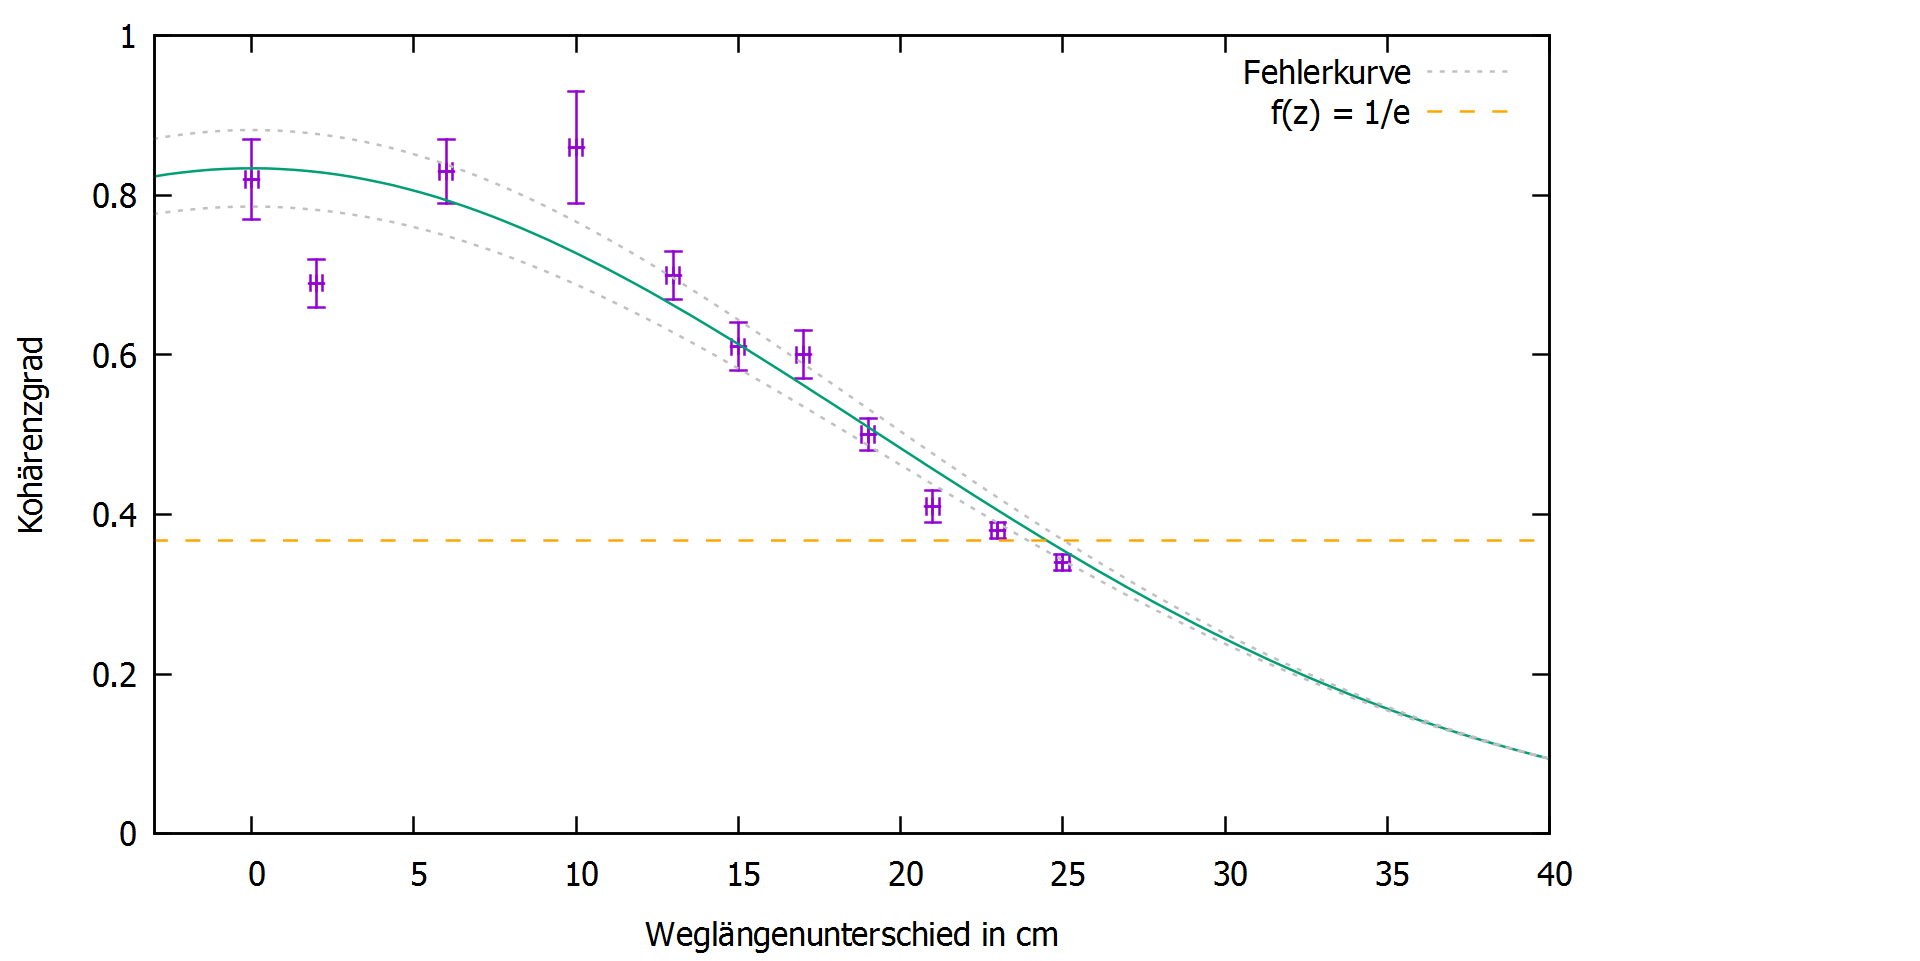
\includegraphics[scale = 0.3]{koplot.png}
	\caption{Kohärenzgrad gegen den Weglängenunterschied der Laserstrahlen im Michelson-Interferometers}
	\label{kopl1}
\end{figure}

\begin{figure}[h]
	\centering
	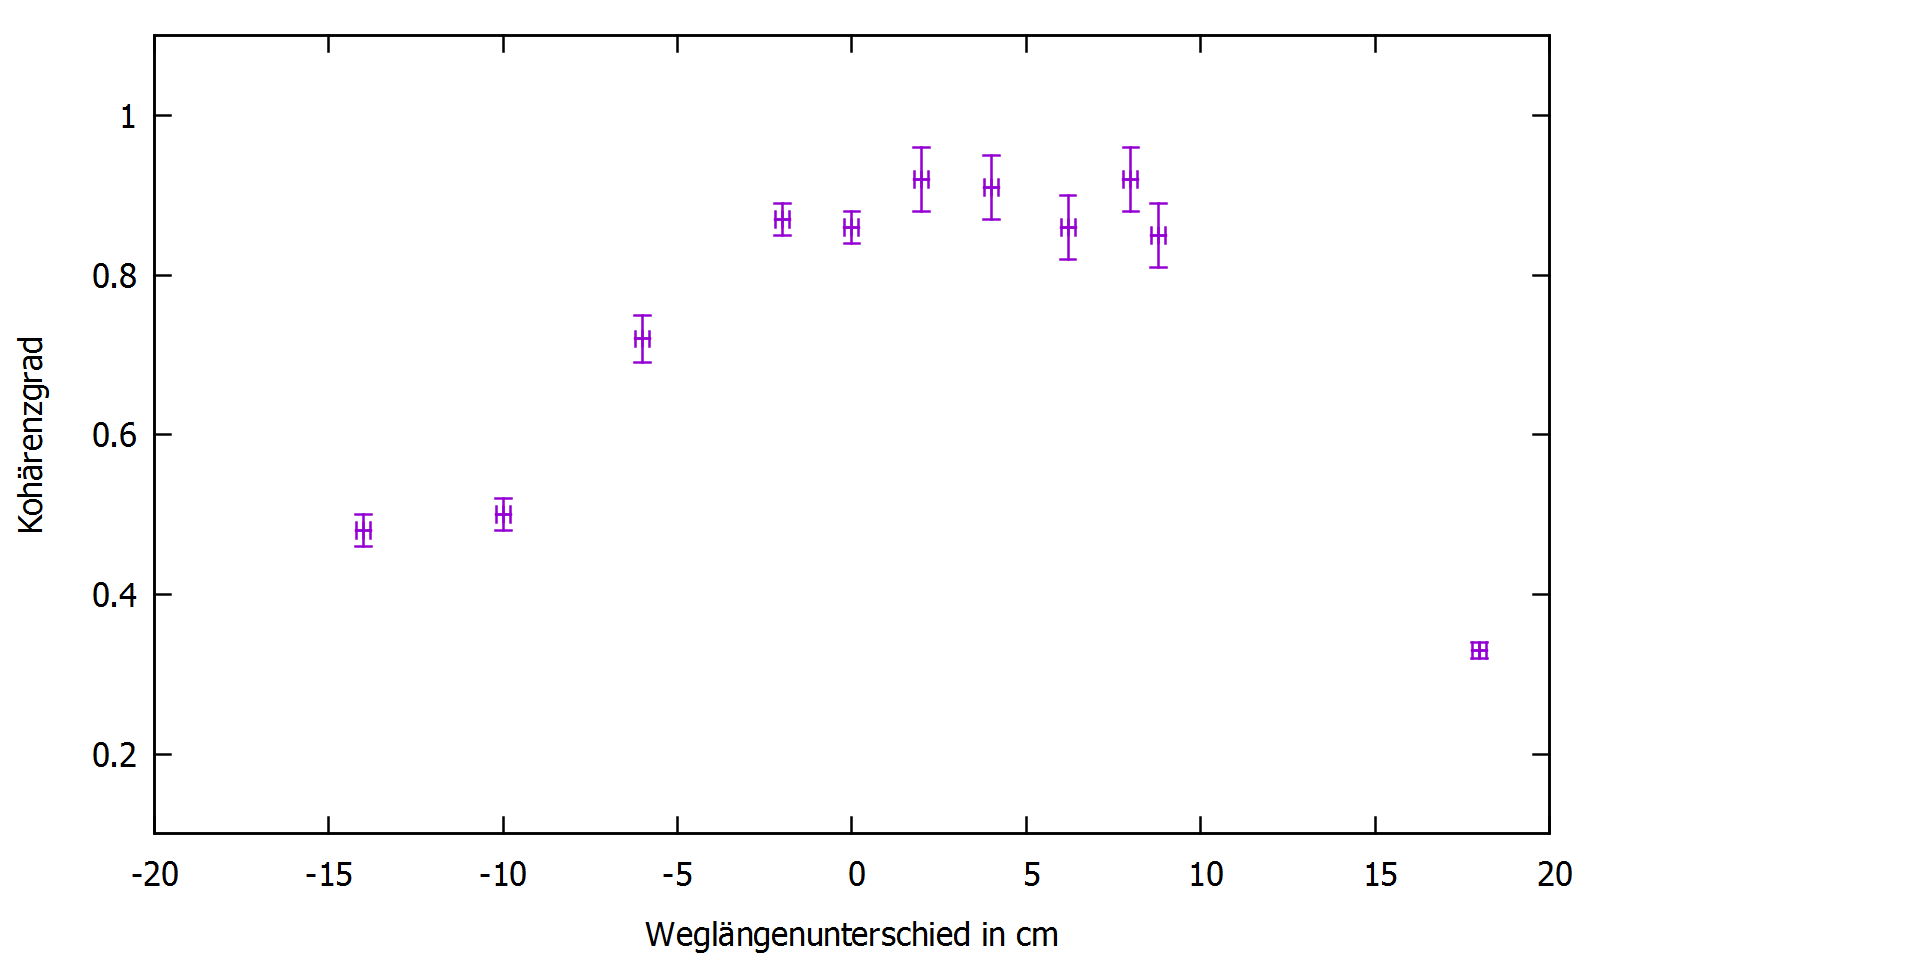
\includegraphics[scale = 0.3]{falsches_koplot.png}
	\caption{Kohärenzgrad gegen den Weglängenunterschied der Laserstrahlen im Michelson-Interferometers für einen falsch herum eingebauten halbdurchlässigen Spiegel}
	\label{kopl2}
\end{figure}

\section{Störungen des Interferenzbildes}

Wir haben die Verschiebung des Interferenzbildes in Abhängigkeit von äußeren Störquellen untersucht. Dazu haben wir die Intensität des Interferenzbildes am festen Ort 45 Sekunden gemessen und währenddessen verschiedene Störungen verursacht. Die Messung kann in Abbildung \ref{stor1} gesehen werden. Während der Messung haben wir neben dem Versuchsaufbau laut geredet und sind umhergelaufen. Zusätzlich haben wir die Tür des Versuchsraums geöffnet und geschlossen und haben kurzzeitig am Untergrund des Versuchsaufbaus gerüttelt. 

Die Störung durch das Rütteln am Untergrund des Versuchaufbaus, kann als Referenz für eine Verschiebung des Interferenzbildes um $\frac{\lambda}{2}$ verwendet werden, da diese Störung sehr intensiv ist. Diese Störung ist in der Abbildung bei $15000ms$ zu sehen. Sie erzeugt eine Spannungsdifferenz von $4V$. Unsere Störungen waren im Vergleich zu den Störungen während der Aufnahme der Hologramme vergleichsweise stark. Über die meiste Zeit der Störungsmessung, von $18000ms$ bis $38000ms$, erzeugen die Störungen eine Spannungsdifferenz im Bereich um $1V$. Das sind $25\%$ der Intensitätsdifferenz von einer Verschiebung um $\frac{\lambda}{2}$. 

Weil wir während der Störungsmessung nahezu durchgehend Störungen erzeugt haben, fällt es schwer die Beruhigungszeit des Aufbaus zu bestimmen. In Abbildung \ref{be1} haben wir zwei Beispiele für eine Beruhigung des Messaufbaus nach einer Störung herausgesucht. Bei \ref{bea} handelt es sich um eine kleine kurzzeitige Störung. Die Störung hat einen Peak bei $11600ms$ und erzeugt eine Spannungsdifferenz von einem Volt. Der Versuchsaufbau benötigt näherungsweise $250ms$ um sich zu beruhigen. In Abb. \ref{beb} kann eine größere Störung, hervorgerufen durch das Rütteln am Untergrund des Versuchsaufbaus gesehen werden. Die Störung ist maximal bei $15000ms$, wo sie eine Spannungsdifferenz von $4V$ erzeugt, und braucht zur Beruhigung bis zur Zeit $17500ms$. Sie hat also eine Beruhigungszeit von $2500ms$. Es fällt auf, dass die Schwankung der Spannung nach $15000$ nicht monoton abnimmt. Dies deutet darauf hin, dass während der Beruhigungszeit der Störung von $15000ms$ eine neue Störung Einfluss auf den Versuchsaufbau nimmt. Dies würde erklären, warum die Beruhigungszeit der Störung aus Abb. \ref{beb} das 10-fache der Beruhigungszeit der Störung aus Abb. \ref{bea} beträgt. 

Aus den beiden Abbildungen lässt sich hauptsächlich erkennen, dass die Beruhigungszeit einer großen Störung länger, als die einer kleinen Störung ist. Zusätzlich lässt sich aus dem Verlauf der Kurven vermuten, dass die Intensität einer Störung während der Beruhigungszeit exponentiell abfällt.

\begin{figure}[h]
	\centering
	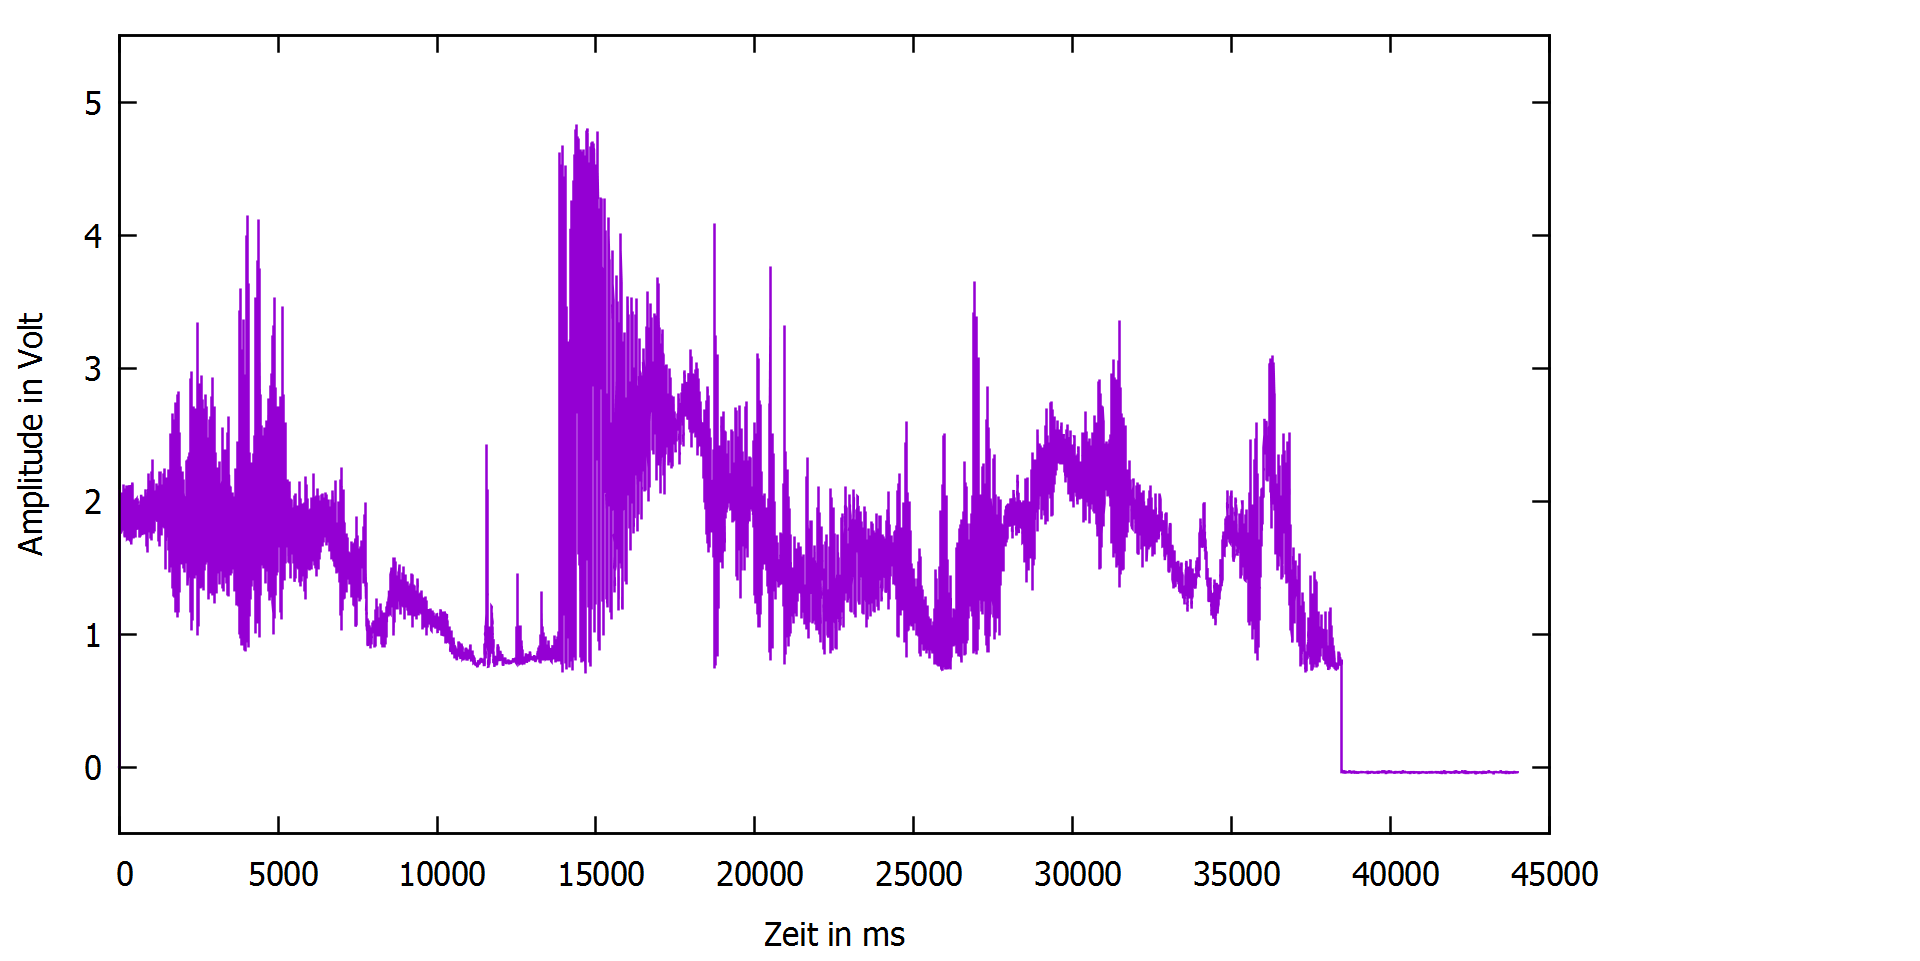
\includegraphics[scale = 0.26]{storung.png}
	\caption{Intensität des Interferenzbildes, aufgetragen gegen die Zeit bei aktiver Erzeugung von Störquellen}
	\label{stor1}
\end{figure}

\begin{figure}[h]
	\centering
	\begin{subfigure}{0.8\textwidth}
		\centering
		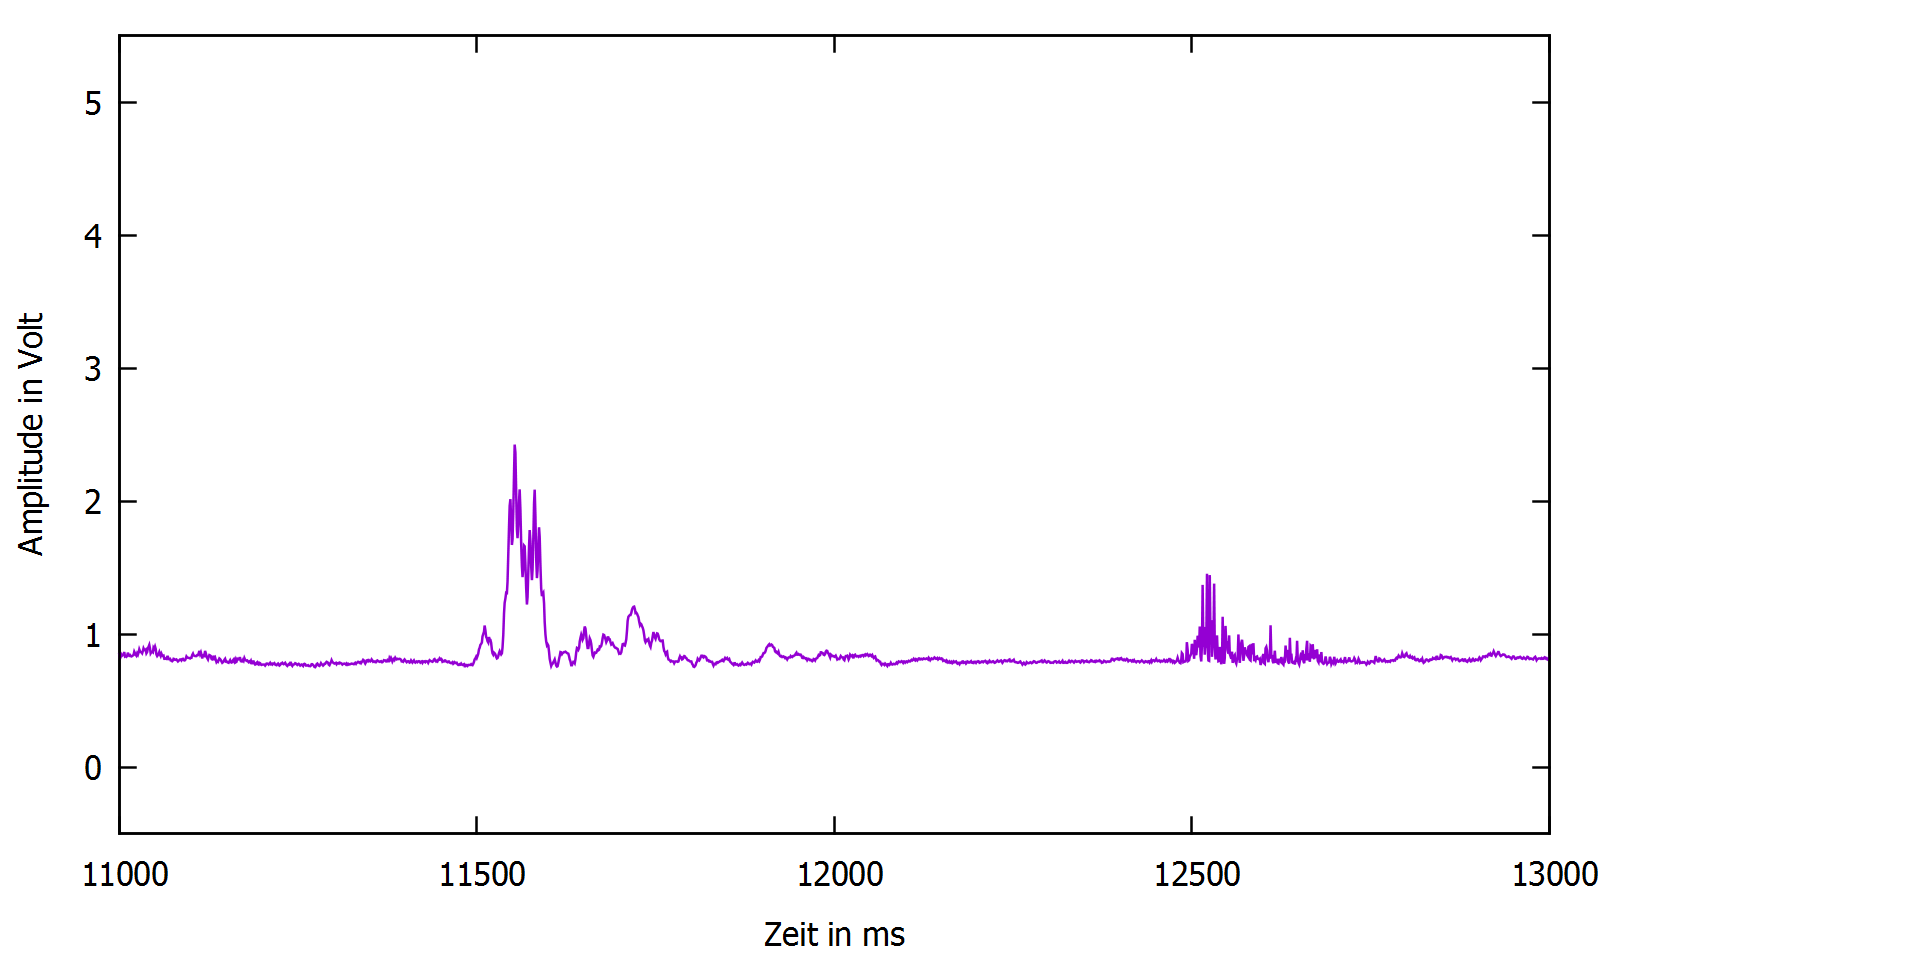
\includegraphics[width=\textwidth]{abklingzeit1.png}
		\caption{kleine kurzzeitige Störung des Messaufbaus}
		\label{bea}
	\end{subfigure}
	\begin{subfigure}{0.8\textwidth}
		\centering
		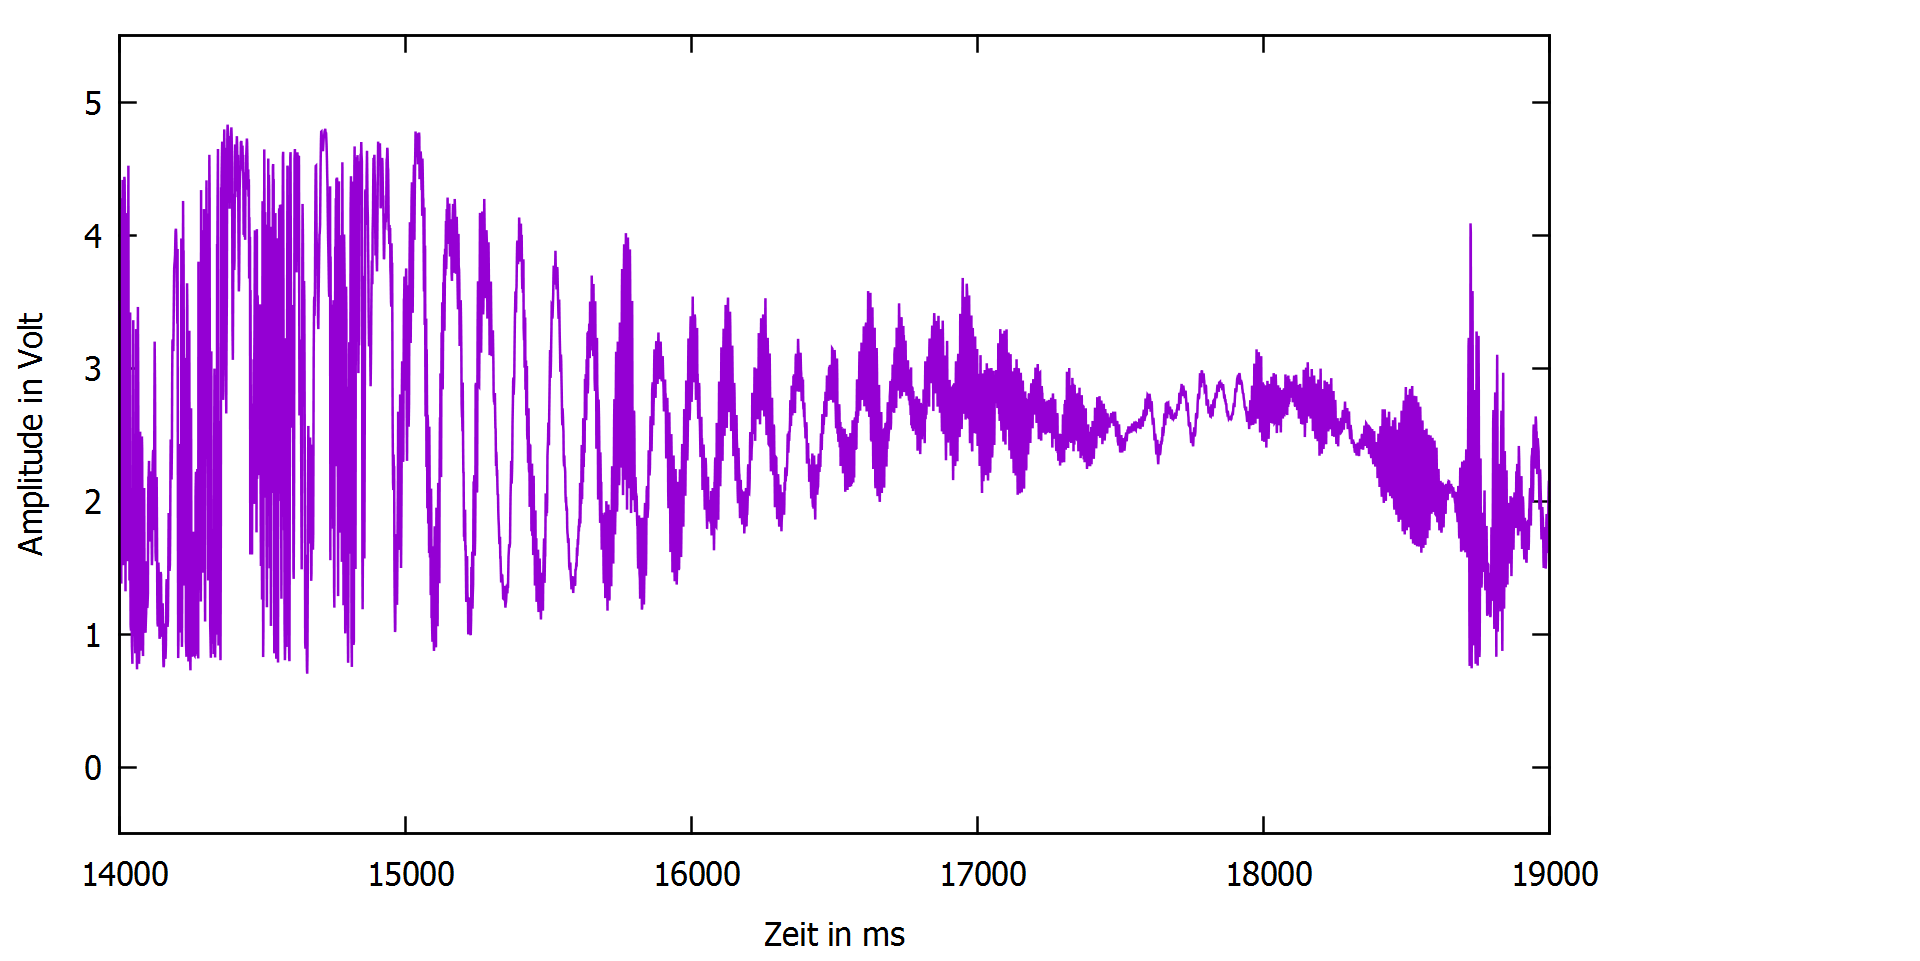
\includegraphics[width=\textwidth]{abklingzeit2.png}
		\caption{Große Störung des Messaufbaus durch Rütteln am Untergrund des Versuchsaufbaus}
		\label{beb}
	\end{subfigure}
	
	\caption{Beruhigung des Messaufbaus nach Störungen}
	\label{be1}
\end{figure}

\section{Diskussion}

Mithilfe eines Michelson-Interferometers haben wir die Kohärenzlänge des von uns verwendeten He-Ne-Lasers auf $(24,5 \pm 0,6)cm$ bestimmt. Diese Länge stimmt mit den theoretischen Werten überein. He-Ne-Laser haben abhängig von ihrer Resonatorlänge oftmals eine Kohärenzlänge zwischen $20cm$ und $30cm$. Die Kohärenz des Lasers genügt, um Hologramme zu erzeugen, da der dafür benötigte Weglängenunterschied zweier Laserstrahlen aus gleicher Quellen kleiner, als die Kohärenzlänge des He-Ne-Lasers ist.

In einer Störungsmessung konnte gezeigt werden, dass der Versuchsaufbau sehr empfindlich gegenüber Störungen ist. Der Grund dafür ist, dass bereits eine kleine Änderung des Weglängenunterschieds der Laserstrahlen im Größenbereich der Wellenlänge des Laserstrahls das Interferenzmuster signifikant verändert. Dies muss bei der Aufnahme von Hologrammen beachtet werden, da diese zur Erzeugung stabile Interferenzmuster benötigen.
Während der Aufnahme der Hologramme durften wir deshalb zum Beispiel nicht sprechen (ebenso musste der Raum abgedunkelt werden). Die Hologramme sind, wie beschrieben, im Allgemeinen gut gelungen.


\section{Quelle}

Abb2 http://www.holografie.com/Fouquier.pdf




\end{document}